\textbf{\underline{OZ 4 - De wet van Ampère en de wet van Biot-Savart - Oefening 2:}}
\vspace{0.5cm}

\begin{minipage}{0.7\textwidth}
    Een circuit bestaat uit twee bogen met straal $R$ en twee rechte stukken op een afstand $2a$ van elkaar. Door het circuit loopt een stroom $I$. Bereken het magneetveld $\vec{B}$ in het punt $P = 0$, gelegen in het vlak van het circuit
    \vspace{1.5cm}
\end{minipage}
\begin{minipage}{0.26\textwidth}
    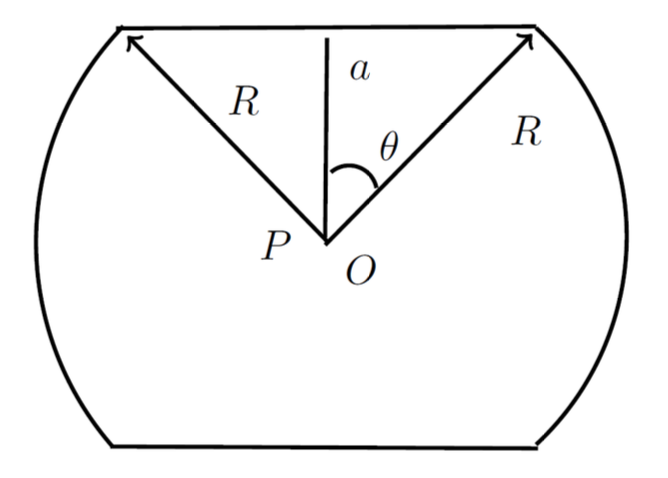
\includegraphics[scale = 0.35]{oz04/resources/Oz4Oef2.png}
\end{minipage}

% \begin{center}
%     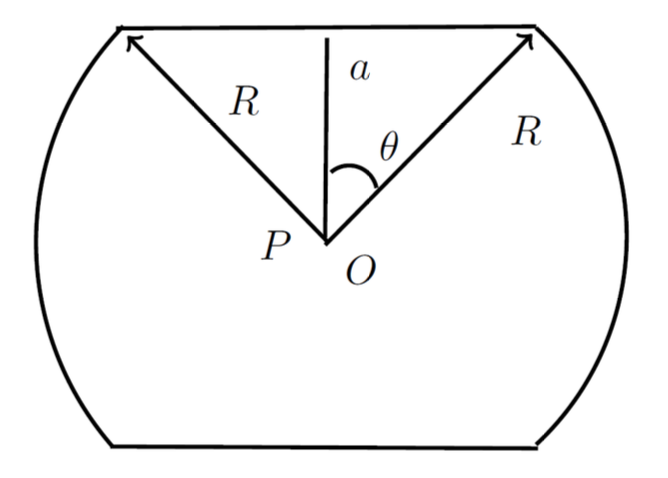
\includegraphics[scale = 0.4]{oz04/resources/Oz4Oef2.png}
% \end{center}
\vspace{-1.5cm}

\begin{description}[labelwidth=1.5cm, leftmargin=!]
    \item[Geg. :]   $R$, $a$, $I$
    \item[Gevr. :]  $\Vec{A}$ ?
    \item[Opl. :]  
    We zullen de vectoriële aanbrenging van de rechte stukken en bogen apart berekenen:
    \begin{itemize}
        \item 
            We berekenen het infinitesimale veld geproduceerd door de rechte stukken
            \begin{align*}
                d\Vec{B}_{|}
                &= \frac{\mu_0I}{4\pi}\frac{d\Vec{\ell}\times\hat{r}}{r^2} \\
                &= \frac{\mu_0I}{4\pi}\frac{d\ell\sin(\phi)}{r^2} \ (\hat{k}) 
            \end{align*}
            waarbij $\phi$ de hoek tussen $d\Vec{\ell}$ en $\hat{r}$ en dit gaan we herschrijven in functie van de hoek $\phi$ 
            \begin{align*}
                d\Vec{B}_{|}
                &= \frac{\mu_0I}{4\pi}\frac{1}{r^2} d\ell\sin(\phi) \ (\hat{k}) \\
                &= \frac{\mu_0I}{4\pi}\frac{\sin^2(\phi)}{a^2} d\ell \sin(\phi) \ (\hat{k}) \\ 
                &= \frac{\mu_0I}{4\pi}\frac{\sin^2(\phi)}{a^2} \frac{a}{\sin^2(\phi)} \sin(\phi) d\phi \ (\hat{k}) \\
                &= \frac{\mu_0I}{4\pi}\frac{1}{a}\sin(\phi) d\phi \ (\hat{k})
            \end{align*}
            waarbij we gebruikt hebben dat
            \begin{equation*}
                \frac{1}{r^2} = \frac{\sin^2(\phi)}{a^2}  \quad \text{en} \quad d\ell = d\left(\frac{a}{\tan(\phi)}\right) = \frac{a}{\sin^2(\phi)}d\phi         
            \end{equation*}
            We integreren hierover om het totale vectoriele veld te vinden van de rechte stukken
            \begin{align*}
                \Vec{B}_{\parallel}
                &= 2\int_{-\phi}^{\phi} d\Vec{B}_{|} \\
                &= \frac{\mu_0I}{2\pi}\frac{1}{a}\int_{-\phi}^{\phi}\sin(\phi)d\phi \ (\hat{k}) \\
                &= \frac{\mu_0I}{\pi}\frac{1}{a}\int_{0}^{\phi}\sin(\phi)d\phi \ (\hat{k}) \\
                &= \frac{\mu_0I}{\pi}\frac{1}{a}\left[-cos(\phi)\right] \ (\hat{k}) \\
                &= \frac{\mu_0I}{\pi}\frac{1}{a}\frac{\sqrt{R^2-a^2}}{R}\ (-\hat{k}) 
            \end{align*}

        \newpage
        
        \item 
            We berekenen het infinitesimale veld geproduceerd door de bogen, we beginnen eerst voor een boog en maken gebruik van $\phi$ van bij de rechte stukken
            \begin{align*}
                d\Vec{B}_{\sim}
                &= \frac{\mu_0I}{4\pi}\frac{d\Vec{\ell}\times\hat{r}}{r^2} \\
                &=  \frac{\mu_0I}{4\pi}\frac{d\ell\sin(\gamma)}{r^2} \ (\hat{k})  \\
                &\overset{\perp}{=} \frac{\mu_0I}{4\pi}\frac{d\phi}{R} \ (\hat{k}) 
            \end{align*}
            waarbij $\gamma$ de hoek is tussen $d\ell$ en $\hat{r}$. 

            Hierover kunnen we integreren en het totale vectoriële veld vinden
            \begin{align*}
                \Vec{B}_{\approx}
                &= 2\Vec{B}_{\sim} \\
                &= \frac{\mu_0I}{2\pi R}\int_{-\phi}^{\phi} d\phi \ (\hat{k}) \\
                &= \frac{\mu_0I}{\pi R}\phi \\
                &= \frac{\mu_0I}{\pi R}\left(\frac{\pi}{2}-\sin^{-1}\left(\frac{\sqrt{R^2-a^2}}{R}\right)\right)
            \end{align*}
            % \textbf{Note:} deze laatste stap is niet echt nodig, ik doe dit slechts om tot de modeloplossing te geraken
    \end{itemize}
    Als we nu de vectoriële som nemen van $\Vec{B}_{\parallel}$ en $\Vec{B}_{\approx}$, vinden we
    \begin{equation*}
        \Vec{B} = \frac{\mu_0I}{\pi R}\left(\frac{1}{a}\sqrt{R^2-a^2} + \frac{\pi}{2} -\sin^{-1}\left(\frac{\sqrt{R^2-a^2}}{R}\right) \right)
    \end{equation*}
    
\end{description}

\vspace{1cm}